%######################Document Setup######################
\documentclass[a4paper, 10pt, titlepage]{article}

\usepackage[pdftex]{graphicx}
\usepackage{anysize}
\usepackage[hidelinks]{hyperref}
\usepackage{float}
\usepackage{fancyhdr}
\usepackage{pdfpages}
\usepackage{amsmath}


\usepackage{paracol}
\setlength{\columnsep}{10pt}

\usepackage{tikz}

\usepackage{xcolor}
\hypersetup{
    colorlinks,
    linkcolor={red!50!black},
    citecolor={blue!50!black},
    urlcolor={blue!80!black}
}

\marginsize{5mm}{5mm}{1mm}{1mm}
\setlength{\parindent}{0pt}
\setlength{\parskip}{1pt}

%################################
\newcommand{\new}[1]{\begin{center}
{\large\textbf{#1}}\end{center}}

\newcommand{\side}[1]{{\small \textbf{\textit{#1:}}}}

\newcommand{\job}[4]{{\normalsize \textbf{#1}} $\bullet$ #3 \\{\small \textit{\textbf{#2}}}\\#4 \\}

\newcommand{\vol}[3]{{\normalsize \textbf{#1}} $\bullet$ #3 \\{\small \textit{#2}}\\}

\newcommand{\point}[1]{$\bullet$ #1\\}
%##########################################################

\begin{document}

%Header
\begin{center}
\begin{LARGE}
\textbf{EEE3069W Formula Sheet}
\end{LARGE} \\ \medskip
\end{center}

\pagenumbering{gobble}

%Content

\begin{paracol}{3}[]
\underline{General} \\
$s^2x + 2 \zeta \omega_0sx + \omega_0^2x$ \\
$g_{CL} = \frac{L}{1+L}$ \\
$ZOH = (1-z^{-1}) = \frac{1 - e^{-sT}}{s}$ \\
$t_{2\%} \simeq 4\tau$ \\
$\zeta = cos(\theta)$ \\
$\tau = \frac{-1}{Re\{s\}} = \frac{1}{\zeta \omega_n}$ \\
$z=e^{sT}=e^{(\sigma + j \omega) T} = e^{\sigma T} e^{j \omega T} = \rho e^\varphi$\\
$t_{2\%}=b:R\{z\}<e^{\frac{-4T}{b}}$\\
\underline{Jury Stability Test} \\
$A(z) = a_0 + a_1z + a_2z^2 + ... + a_nz^n = 0$ \\
$A(1)>0$, $A(-1)>0$ for n even, $A(-1)<0$ for n odd. \\
$|a_0|<|a_n|$, $|b_0|>|b_{n-1}|$, $|c_0|>|c_{n-2}|$, ... \\
where $b_k = \begin{vmatrix}
a_0 & a_{n-k}\\
a_n & a_k\\
\end{vmatrix}$, ... \\
\underline{Z-Transform}
$$Z[x(kT)] = \sum^{\infty}_{k=0} x(kT)z^{-k}$$ 
$$\sum^{\infty}_{k=0} r^k = \frac{1}{1-r}$$
$e^{j\theta} = cos(\theta) + jsin(\theta)$ \\
$sin(\theta) = \frac{e^{j\theta} - e^{-j\theta}}{2j}$ \\
\underline{Sampling} \\
$g^*(s) = g(z)$ \\
$g^*(t) = g(nT)$ \\
$y(s)=g(s)u(s);y^*(s)=gu^*(s);$\\
$y(z)=gu(z)$\\
$\frac{y(z)}{r(z)}$: pulse transfer function.\\
$u^*(s+jm\Omega) = u^*(s);\Omega = \frac{2\pi}{T};$\\
$\Omega/2>BW$\\
\underline{Controllability and Observability} \\
$\frac{d}{dt} x(t) = Ax(t) + bu(t)$ \textit{with n states.} \\
$y(t) = C^Tx(t) + du(t)$ \\
C: $Rank[b|Ab|A^2b|...|A^{n-1}b] = n$ \\
O: $Rank[C^T|C^TA|C^TA^2|...|C^TA^{n-1}]^T = n$ \\
\textit{where R(rows) = R(columns) = LI columns / no. of pivots / no. zero rows in RRE form.} \\
\textit{Can you 'see' control action (u(t)) and output?}\\
$x=P\bar{x}; P^{-1}AP = D$ \\
\underline{Discrete Controller Implementation} \\
\textbf{\textit{Difference equation:}} \\
$k(z) = \frac{u(z)}{e(z)};u(z)z^{-a} = u(n-a)$ \\
\textbf{\textit{Direct:}} powers of $z^{-1}$; introduce internal state variable x(z); equate denominator then numerator; no. past values = no. poles \\
\textbf{\textit{Cascade:}} split into first order blocks connected in cascade; apply direct; use internal variables to equate \\
\textbf{\textit{Parallel:}} partial fraction expansion; apply direct; use internal variables to equate \\
$e(z)\Rightarrow k(z) \Rightarrow u(z)$ \\

\switchcolumn 
\underline{State Feedback Control} \\
$u(t) = -k^Tx(t) + r(t)$ \\
\textit{Replace u(t) in basic state space model and take Laplace:} \\
$g(s) = \frac{y}{r} = C^T \frac{(sI-A+bk^T)b}{det(sI-A+bk^T)}$ \\
$\phi_c = det(sI-A+bk^T)$ \\ 
$det(sI-A+bk^T) = 0$ \\ 
\textit{for closed-loop poles = eigenvalues of $(\bar{A} = A - bk^T)$.} \\

\textit{\textbf{Set-point tracking:}} \textit{add K/s, block diagram manipulation, state space for integrator:} \\
$\frac{d}{dt}x_a = r(t) - C^Tx(t) +du(t)$ \\
$z=-k_ax_a$ \\
\textit{Integrator output becomes a state and augmented matrix formed:} \\
$\frac{d}{dt}
\begin{bmatrix}
x\\x_a
\end{bmatrix}
= 
\begin{bmatrix}
A & 0\\
-C^T & 0\\
\end{bmatrix}
\begin{bmatrix}
x\\x_a
\end{bmatrix}
+
\begin{bmatrix}
b\\-d
\end{bmatrix}
u
+
\begin{bmatrix}
0\\1
\end{bmatrix}
r
$\\
$u(t) = -\begin{bmatrix}
k^T & k_a
\end{bmatrix}
\begin{bmatrix}
x \\ x_a
\end{bmatrix}$
\textit{subbing this in gives:} \\
$\frac{d}{dt}
\begin{bmatrix}
x\\x_a
\end{bmatrix} =
(\bar{A} - \bar{b}\bar{k}^T) \begin{bmatrix}
x \\ x_a
\end{bmatrix}
+ \begin{bmatrix}
0 \\ 1
\end{bmatrix} r$ \\
$\phi_c = |sI-\bar{A} + \bar{b}\bar{k}^T|$ \\

\textbf{\textit{Observer:}} \textit{the observer state is added and error poles can be designed separately from CL poles:} \\
$\frac{d}{dt}\tilde{x}(t) = A\tilde{x}(t) + bu(t) + p[y(t)-\tilde{y}(t)]$\\
$\tilde{y}(t) = C^T\tilde{x}(t)$\\
\textit{state observer is a mathematical model of plant with error term. $\tilde{x}(t)$ is an estimated state.} \\
\textit{Introducing error state:} \\
$\frac{d}{dt}e = x - \bar{x} = (A-pC^T)e$ \\
$\begin{vmatrix}
sI-A+bk^T
\end{vmatrix}
\begin{vmatrix}
sI-A+pC^T
\end{vmatrix}
= 0
$ \\

\switchcolumn 
\underline{Modified Z-Transform} \\
$Z_m[gh(s)] = Z[gh(s)e^{-s\theta}]$\\
$m=1-\frac{\theta}{T}=1-\Delta$\\

\underline{Other Transformations} \\
$z=\frac{1+w}{1-w}$\\
$w=\frac{z-1}{z+1}$\\

$z=\frac{1+w'\frac{T}{2}}{1-w'\frac{T}{2}}$\\
$w'=\frac{2(z-1)}{T(z+1)}$\\
\textit{Used for: Nyquist of gh(z)}\\

$z=e^{j\omega T}$\\
$w=\frac{e^{j\omega T}-1}{e^{j\omega T}+1} = jtan(wT/2) \simeq j\omega T/2 \simeq j\Omega$\\

\underline{Root Locus} \\
$n_\infty = n_p - n_z$ \\
$angle = \frac{180^0 - 360^0l}{n_\infty}$ \\
$center = \frac{sum of poles - sum of zeros}{n_\infty}$ \\
\textit{Symmetric about real axis.}\\
\textit{Left of odd number of poles and zeros.}\\
$q(s)=\gamma \frac{N_q(s)}{D_q(s)}$\\
$\frac{d}{ds}\gamma(s) = N_q(s)\frac{d}{ds}D_q(s)-D_q(s)\frac{d}{ds}N_q(s)=0$\\
\textit{Between open loop poles - breakaway point.}\\

\underline{Controller Synthesis}\\
$k(z)=\frac{1}{gh(z)}\cdot \frac{\frac{y(z)}{r(z)}}{1-\frac{y(z)}{r(z)}}$\\
\textbf{Dalin:} $\frac{z^{-N}(1-e^{\frac{-T}{\tau}})}{z-e^{\frac{-T}{\tau}}}$\\

\end{paracol}

%\newpage
%\begin{center}
%\begin{LARGE}
%\textbf{EEE4093F Formula Sheet}
%\end{LARGE} \\ \medskip
%\end{center}
%
%\begin{paracol}{3}[]
%
%\switchcolumn
%
%\switchcolumn
%
%\end{paracol}

\newpage
\begin{paracol}{2}[]
\medskip \medskip
\begin{figure}
\begin{center}
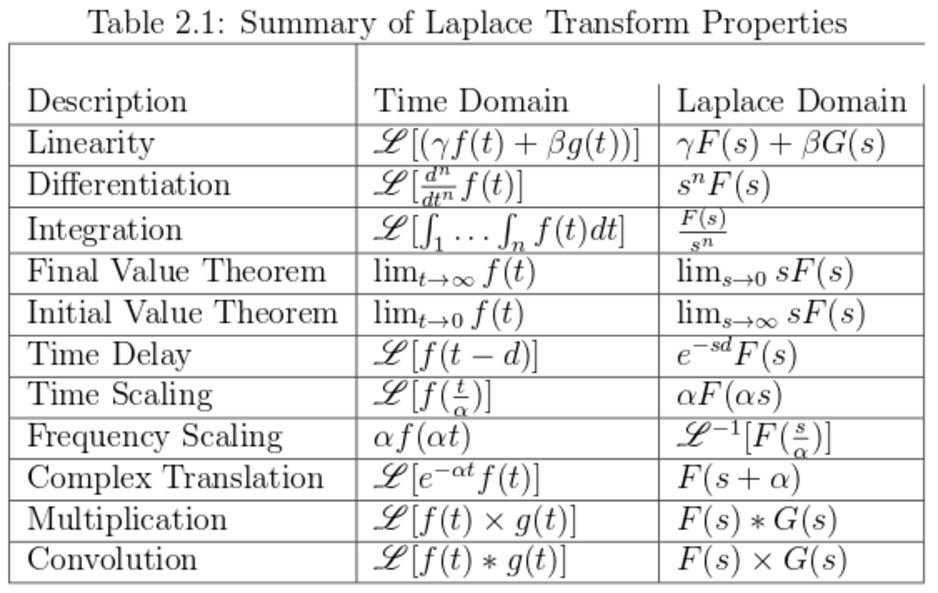
\includegraphics[scale=0.5]{laplace-properties.pdf}
\end{center}
\end{figure}

\begin{figure}
\begin{center}
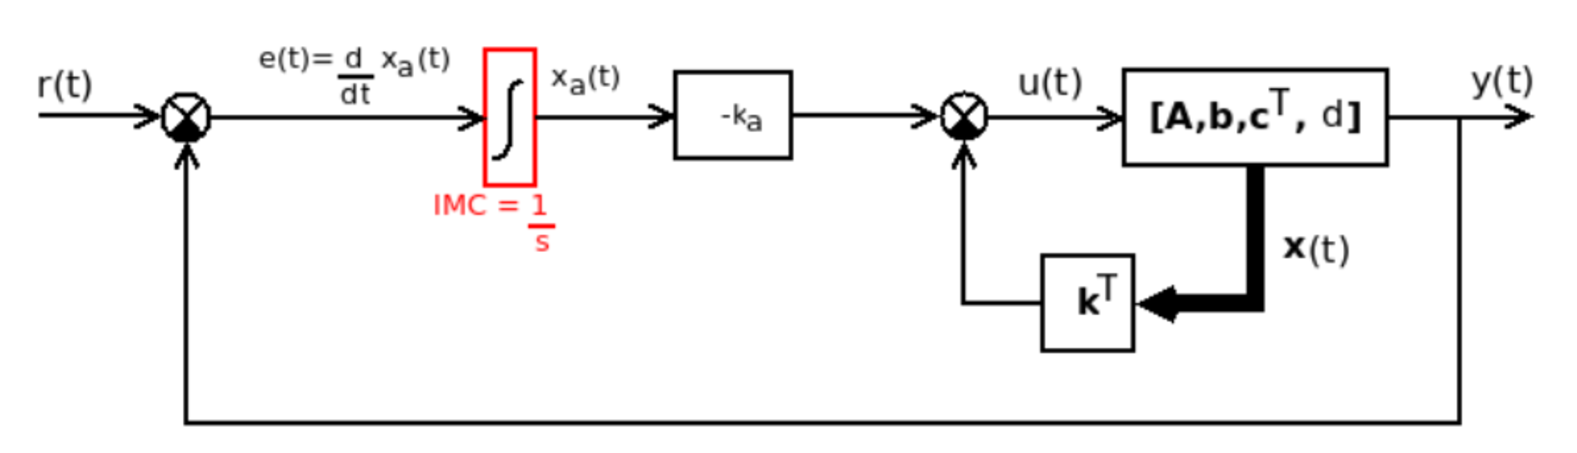
\includegraphics[scale=0.3]{setpoint-statef.pdf}
\end{center}
\end{figure}

\begin{figure}
\begin{center}
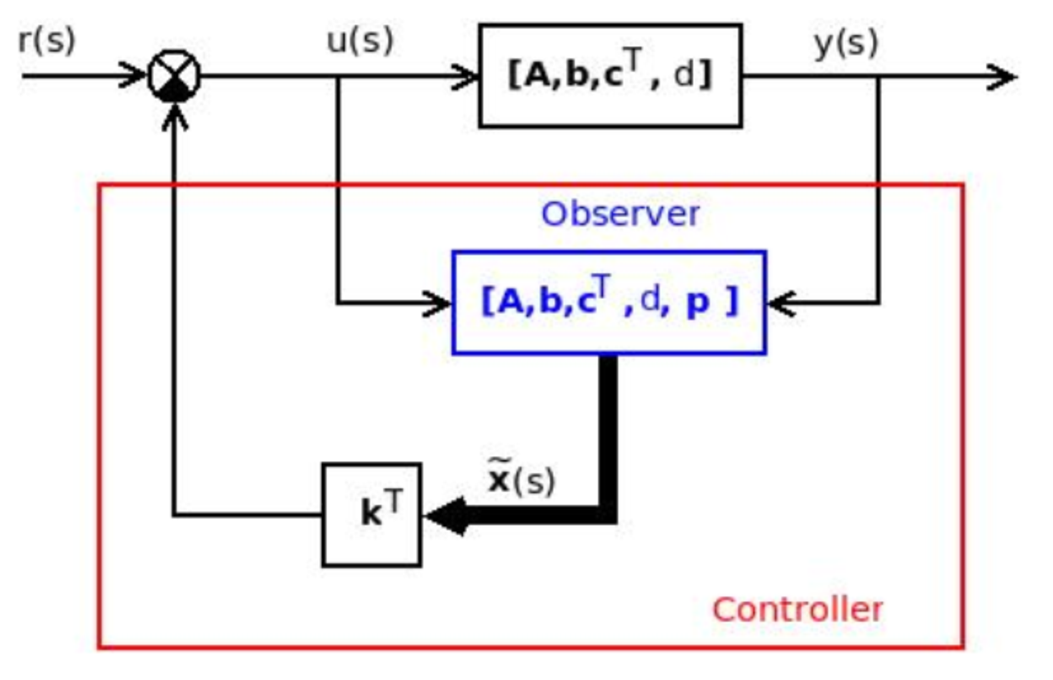
\includegraphics[scale=0.4]{observer-statef.pdf}
\end{center}
\end{figure}

\end{paracol}

\newpage

\pagestyle{fancy}
\fancyhf{}
\chead{\cite{z-transform}}
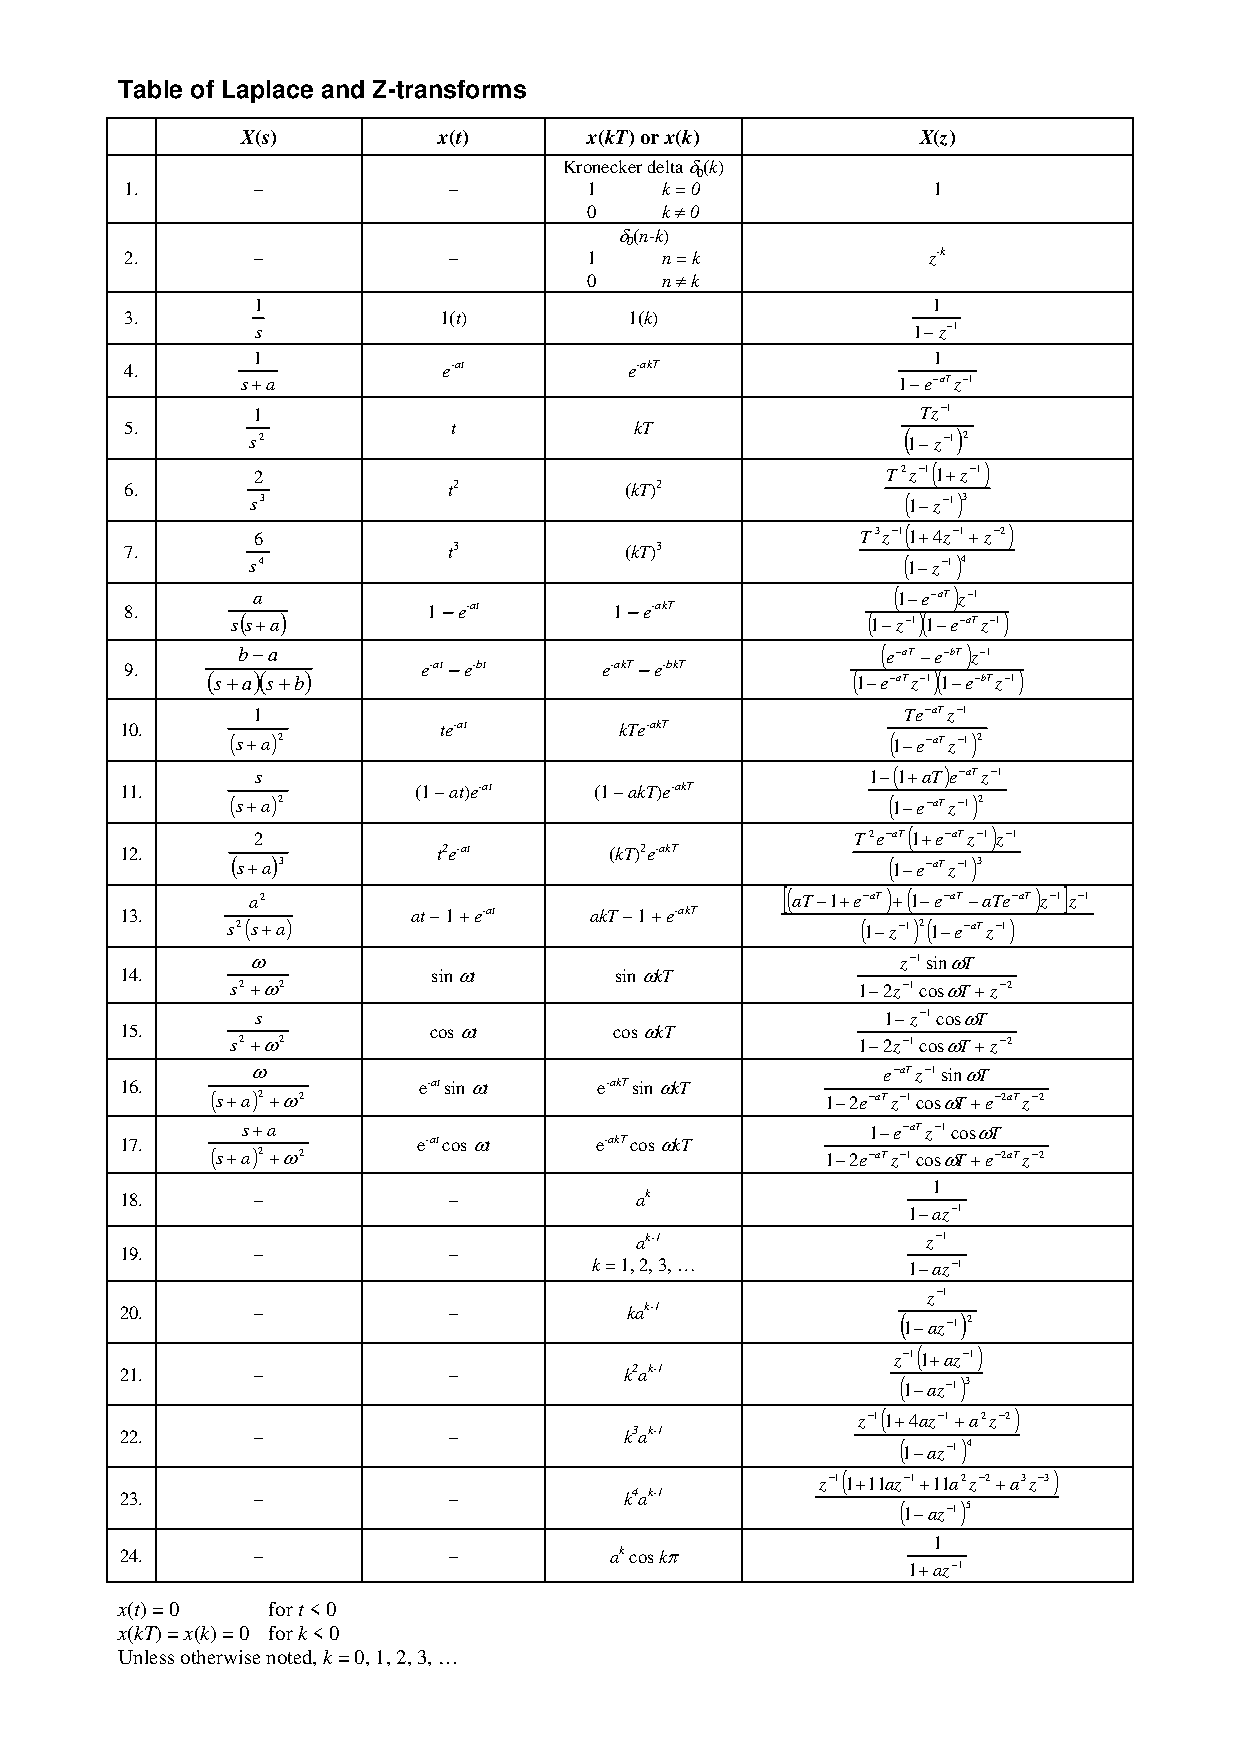
\includepdf[pages=-, scale=1]{TabellaTrasformataZ.pdf}

\bibliography{bibliography}
\bibliographystyle{ieeetran}

\section*{Contributors}
Benjamin Scholtz\\
Sean Wood



%\begin{paracol}{2}[]


%\begin{tabular}{l l l}
%  \textbf{Year}&\textbf{Duration}&\textbf{Description}\\
%  2015 & 1m & \\
%  2006 & 8 \\
%\end{tabular}

%\switchcolumn

%\end{paracol}

\end{document}